\documentclass{article}
\usepackage[utf8]{inputenc}
\usepackage{amsmath}
\usepackage{amsthm}
\usepackage{graphicx}
\usepackage[english]{babel}

% path to images
\graphicspath{ {../graphs/} }
\usepackage[left=2cm,right=2cm,
    top=2cm,bottom=2cm,bindingoffset=0cm]{geometry}
\title{AutomataGroups}
\author{davendiy }
\date{March 2020}

\newtheorem{definition}{Definition}[section]

\newtheorem{statement}{Statement}[section]

\newtheorem{theorem}{Theorem}[section]
\newtheorem{lemma}[theorem]{Lemma}

\begin{document}

% \maketitle

\section{The worst case}

*Here should be definition of the group $G$*

\theoremstyle{definition}
\begin{definition}
	 Function $\textbf{size} : G \rightarrow \mathbf{N} \cup \{0\}$ is defined recursively:
	
	\begin{equation} 
	size(w = \pi (w_1, w_2, w_3)) =
	\begin{cases}
	0, \quad  w = e \\
	0, \quad  w = \delta \quad \text{(reverse node)} \\
	|w| + size(w_1) + size(w_2) + size(w_3)\text{,} \quad \text{otherwise}
	\end{cases}
	\end{equation}
\end{definition}



Thus, $size(a) = size(b) = size(c) = 1$ by definition.

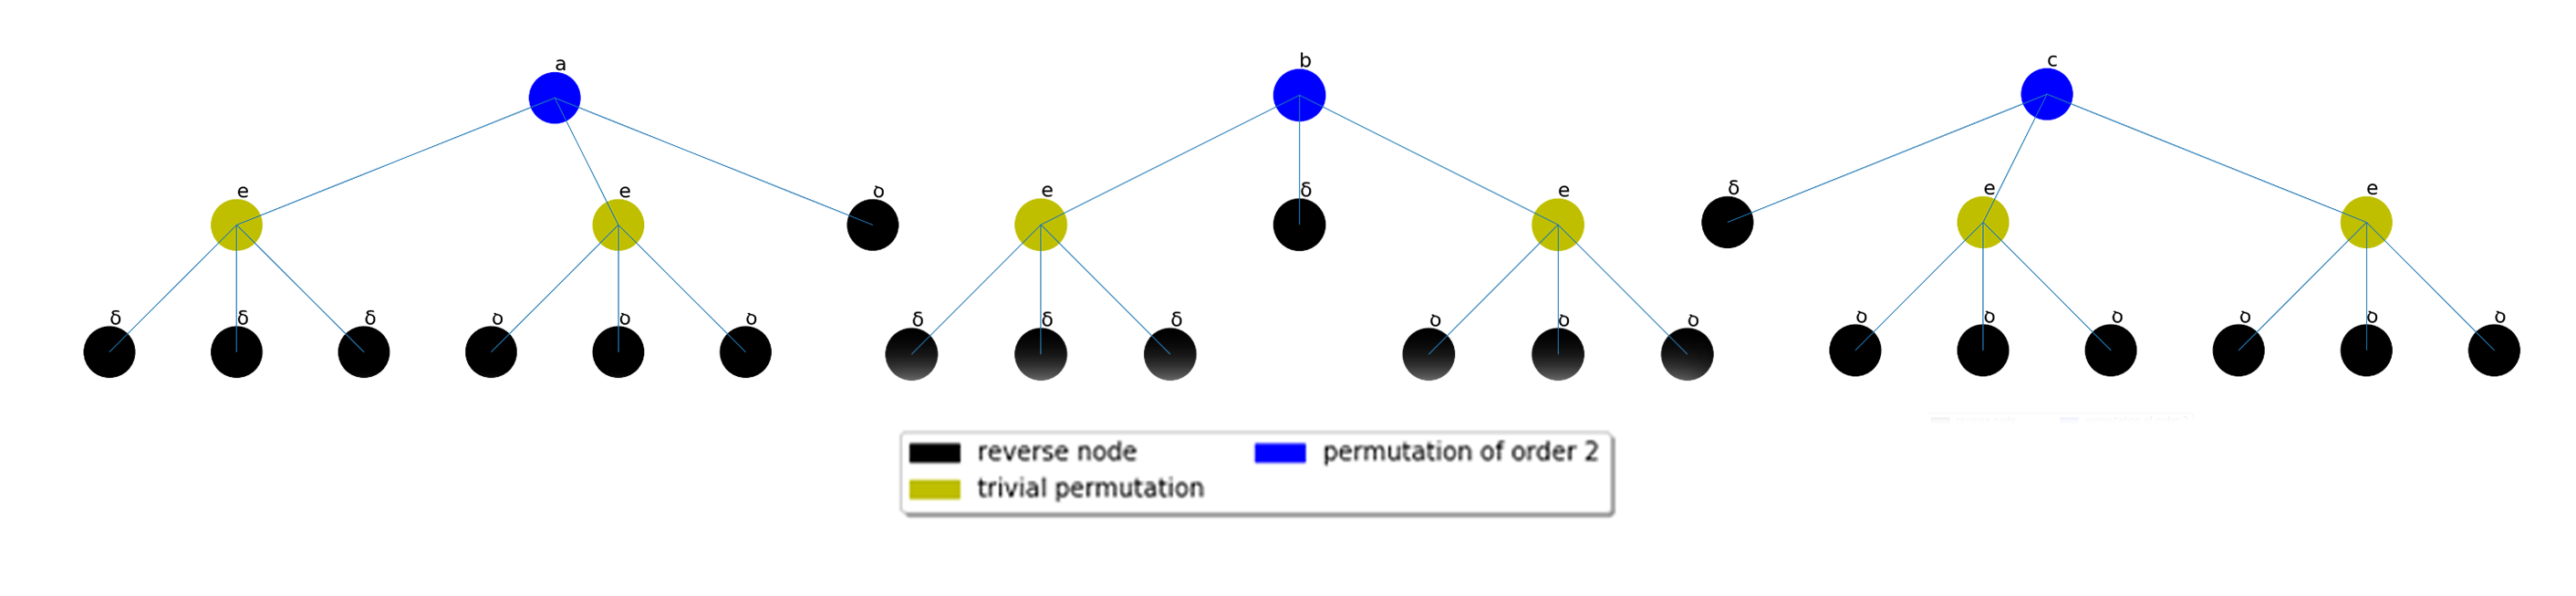
\includegraphics[scale=0.13]{../graphs/a_b_c.png}


Similarly, $size(aa) = size(bb) = size(cc) = 2, \quad size(ab) = size(ac) = ... = size(bc) = 4$

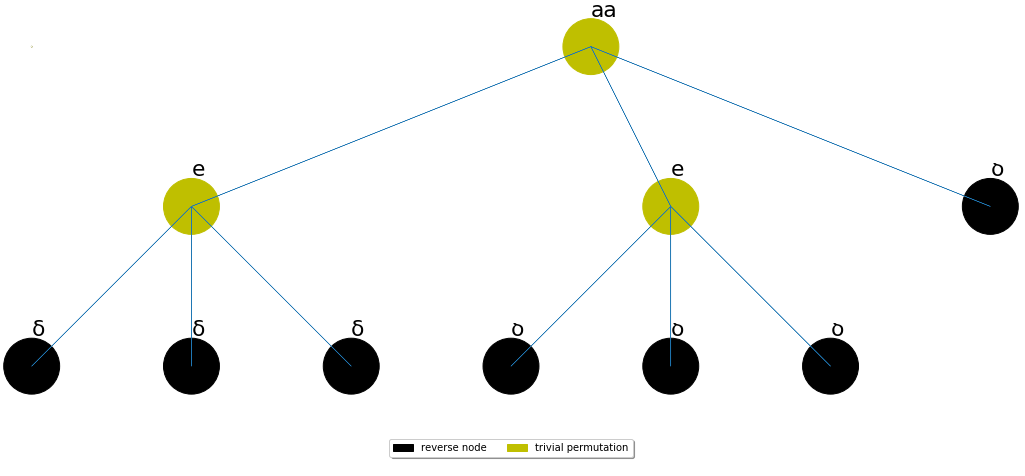
\includegraphics[scale=0.25]{../graphs/aa.png}
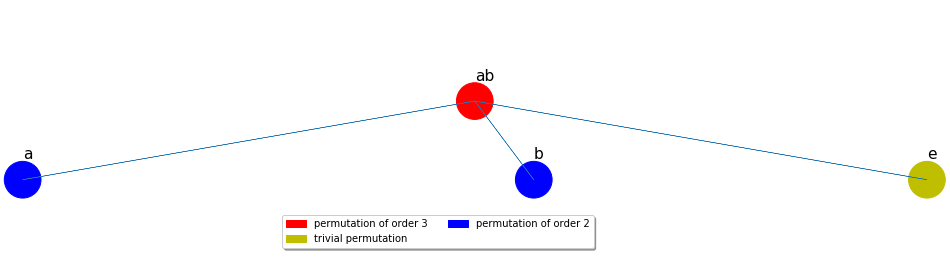
\includegraphics[scale=0.25]{../graphs/ab.png}

\begin{definition}
	\textbf{abc-subset} $X \subset  \{a, b, c\}^*$ is such subset: 
	
	\begin{equation}
		 X = \left\{ (a^\pi b^\pi c^\pi)^k, \, (a^\pi b^\pi c^\pi)^k a^\pi, \, (a^\pi b^\pi c^\pi)^k a^\pi b^\pi  |\, k \in \mathbf{N}\cup\{0\}, \, \pi \in S_3   \right\}
	\end{equation}
	where $a^\pi$ means $S_3$ group action on set $\{a, b, c\}$; \\
	$(w_1 w_2 w_3)^k$ means repeating $k$ times of the expression in the parenthesis.
	\\
	
\end{definition}

\begin{lemma}
	$\forall w \in X \, w$ will have one of the next possible structures:
	$$\pi (w_1, w_2, e), \quad \pi(w_1, e, w_2), \quad \pi(e, w_1, w_2), $$
	where $w_1, w_2 \in X, \quad |w_1|, |w_2| \in
	\left\{
	\left\lfloor
	\frac{n}{2}
	\right\rfloor,
	\left\lceil
	\frac{n}{2}
	\right\rceil
	\right\}, \quad |w_1| + |w_2| = n, \quad n = |w|$
	\\
\end{lemma}

\begin{proof}
	Follows from definition of multiplication.
\end{proof}

Example: 

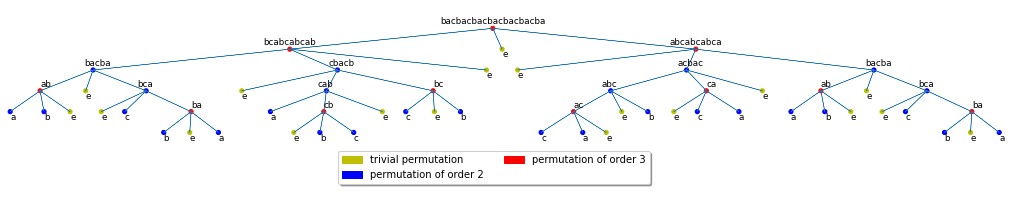
\includegraphics[scale=0.5]{../graphs/max_size_tree.png}

Therefore, here we have recursive formula for calculating function $size$ \textbf{(1)} for elements from $X$:

$$size(w \in X) = a (n) = a \left(
    \left\lfloor
        \frac{n}{2}
    \right\rfloor
\right)
+ a \left(
    \left\lceil
        \frac{n}{2}
    \right\rceil
\right) + n, \quad a(1) = 1, \quad a(0) = 0, \quad n = |w|
$$

\begin{statement}
	Exact form of function $a(n)$:
	\begin{equation}
		 a(n) = \begin{cases}
		 n \left(\left\lfloor \log_2 n + 1 \right\rfloor\right) + 2n - 2^{\left\lfloor\log_2 n\right\rfloor + 1}, \quad n > 0 \\
		 a(0) = 0
		 \end{cases}
	\end{equation}
\end{statement}

\begin{proof}
	$$ a (n+1) = n + 1 + a \left(
	\left\lfloor 
	\frac{n+1}{2}
	\right\rfloor 	
	\right)  + a \left(
	\left\lceil 
	\frac{n+1}{2}
	\right\rceil 
	\right) = n + 1 + a \left(
	\left\lfloor 
	\frac{n}{2} 
	\right\rfloor + 1
	\right) + a \left(
	\left\lceil 
	\frac{n}{2}
	\right\rceil 
	\right)
	$$
	
	$$\text{Let} \, b(n) := a(n + 1) - a(n) = 1 + a \left(
	\left\lfloor
	\frac{n}{2}
	\right\rfloor + 1
	\right) - a \left(
	\left\lfloor
	\frac{n}{2}
	\right\rfloor
	\right) \, \text{ - auxiliary recursion.
	}
	$$
	
	$$ b(n) = b\left(
	\left\lfloor
	\frac{n}{2}
	\right\rfloor
	\right) + 1, \quad b(2) = 4 \quad \Rightarrow \quad b(n) = \left\lfloor \log_2{n}\right\rfloor + 3
	$$
	
	$$
	a (n + 1) = b(n) + b(n-1) + ... + b(1) = 
	\sum_{1 \le k \le n} \left(
	\left\lfloor
	\log_2{k} + 3
	\right\rfloor	
	\right) \quad \Rightarrow \quad a(n) = 2(n - 1) + 
	\sum_{1 \le k \le n} \left(
	\left\lfloor
	\log_2{k} + 1
	\right\rfloor	
	\right)  = 
	$$
	$$
	= \begin{bmatrix}
	\text{amount of bits in all the} \\
	\text{numbers from} \,1 \,\text{to} \,N-1
	\end{bmatrix} = 2(n-1) + \sum_{i=1}^{\left\lfloor\log_2 n\right\rfloor} (n - 2^i) = n \left(
	\left\lfloor
	\log_2 n + 1
	\right\rfloor 
	\right) + 2n - 2^{\left\lfloor\log_2 n\right\rfloor + 1}
	$$
\end{proof}


\begin{theorem}
 	Elements from abc-subset X have maximum size, or in other words 
 	$$a (n) = \max (size(w) \,|\, w \in \{a,b,c\}^n)$$
\end{theorem}

\begin{proof}
	Induction on $n$.
	\begin{enumerate}
		\item Base: check examples of size calculation.
		\item Induction step:\\ 
		Let $\forall k < n \quad a (k) = \max (size(w) \,|\, w \in \{a,b,c\}^k)$. Hereafter we consider any $w \in \{a, b, c\}^{n}, \,\\ w = \pi (w_1, w_2, w_3), \, w_1, w_2, w_3 \in \{a, b, c\}^*\cup \{e\}$. Now we need to show that $size(w) \le a(n)$\\
		\\
		Let $ x_1 := |w_1|, \, x_2 := |w_2|, \, x_3 := |w_3|$. If $w$ has maximum size than due to induction hypothesis \\ 
		\begin{equation}
			size(w) \le a(x_1) + a(x_2) + a(x_3) + n
		\end{equation}
		 (we don't know whether any $w_1, w_2, w_3$ from $X$ could appear in $w$, so we use $\le$ symbol). Let's investigate how big this functional could be.\\
		\\
		Consider function $f(x) = x\log_2{x}$ instead of $a(x)$. We can do it because both $f(x)$ and $a(x)$ are monotonically increasing on $x \ge 1$. Thus, they are maximizing in similar way.
		\\
		Now we need to solve optimization problem 
		$$\max(f(x_1) + f(x_2) + f(x_3) \, | x_1>1,\, x_2>1,\, x_3>1,\, x_1 + x_2 + x_3 = n)$$
		$$F = f(x_1) + f(x_2) + f(x_3) = x_1 \log_2 x_1 + x_2 \log_2 x_2 + x_3 \log_3 x_3 = \Big[x_3 = n - x_1 - x_2\Big] =$$
		$$ = x_1 \log_2 x_1 + x_2 \log_2 x_2 + (n - x_1 - x_2) \log_2 (n-x_1 - x_2) = $$
		$$= x_1\log_2 x_1 + x_2 \log_2 x_2 + n \log_2 (n - x_1 - x_2) - x_1 \log_2 (n - x_1 - x_2) - x_2 \log_2(n - x_1 - x_2)$$
		$$\frac{\partial F}{\partial x_1} = \log_2 x_1 + \frac{1}{\ln 2} - \frac{n}{(n - x_1 - x_2)\ln 2} - \log_2 (n - x_1 - x_2) + \frac{x_1}{(n-x_1 - x_2)\ln 2} + \frac{x_2}{(n - x_1 - x_2) \ln 2}$$
		$$\frac{\partial F}{\partial x_2} = \log_2 x_2 + \frac{1}{\ln 2} - \frac{n}{(n - x_1 - x_2)\ln 2} - \log_2 (n - x_1 - x_2) + \frac{x_1}{(n-x_1 - x_2)\ln 2} + \frac{x_2}{(n - x_1 - x_2) \ln 2} $$
		If both $\dfrac{\partial F}{\partial x_1}$ and $\dfrac{\partial F}{\partial x_2}$ equal to zero then $\log_2 x_1 = \log_2 x_2 \, \Rightarrow \, x_1$ should be equal to $x_2$.
		\\
		Let's substitute $x = x_1 = x_2$ to F and differentiate it: 
		
		$$\frac{d F}{d x} = 2\log_2 x + \frac{2}{\ln 2} - \frac{2n}{(n-2x)\ln2} - 2\log_2 (n - 2x) + \frac{4x}{(n-2x)\ln 2} = 0$$
		Hence, $x = \dfrac{n}{3}$ - the single solution (Wolfram).
		Substituting it to $F$ we can find out that $x_1 = x_2 = x_3 = \dfrac{n}{3}$ - global minimum. Thus, F (therefore right part of \textbf{(4)}) reaches its maximum value on the bounds of its domain. 
		\\
		Now we are allowed to assume that $\exists i \, w_i = e$, because we know that otherwise
		$$size(w) \le a(x_1) + a(x_2) + a(x_3) + n \le a\left(
			\left\lfloor
				\frac{n}{2}
			\right\rfloor 
		\right) + a \left(
			\left\lceil
			\frac{n}{2}
			\right\rceil
		\right) + n$$
		It's easy to check that there are only 2 possible types of $w$ with one or more trivial element below: familiar to us $w \in X$ or such $w = z_1 z_2 z_3 ... z_n$ where there are at least one $i$ such that $z_i = z_{i+1}, \, \Rightarrow \, w$ could be reduced $\Rightarrow$ $size(w) < a(n)$ due to definition.
 	\end{enumerate}

\end{proof}


\section{Generative function}

$$ T(z) = \sum_{w}size(w)z^{|w|} = \sum_{w_1}\sum_{w_2}\sum_{w_3}\left(s(w_1) + s(w_2) + s(w_3) +|w_1| + |w_2| + |w_3|\right)z^{|w_1| + |w_2| + |w_3|} =$$
$$=\sum_{w_1}\sum_{w_2}z^{|w_1| + |w_2|}\left((s(w_1) + s(w_2))\sum_{w_3}z^{|w_3|} + \sum_{w_3}s(w_3)z^{|w_3|} + (|w_1| + |w_2|)\sum_{w_3}z^{|w_3|} + \sum_{w_3}|w_3|z^{|w_3|}\right) = $$
$$= \left[\sum_{w}z^{|w|} = F(z), \quad \sum_{w}|w|z^{|w|} = z\sum_{w}|w|z^{|w| - 1} = zF'(z)\right] = $$
$$=\sum_{w_1}z^{|w_1|}\sum_{w_2}z^{|w_2|}\left((s(w_1) + s(w_2) + |w_1| + |w_2|)F(z) + T(z) + zF'(z)\right) = $$
$$ = \sum_{w_1}z^{|w_1|}\left(
			(T(z) + zF'(z))\sum_{w_2}z^{|w_2|} + F(z) \left( (s(w_1) + |w_1|)\sum_{w_2}z^{|w_2|} + \sum_{w_2}s(w_2)z^{|w_2|} + \sum_{w_2}|w_2|z^{|w_2|} \right)
\right) = $$
$$ = \sum_{w_1}z^{|w_1|} \left[ (T(z) + zF'(z))F(z) + F(z) ( (s(w_1) + |w_1|)F(z) + T(z) + zF'(z)) \right]  = $$
$$= \sum_{w_1}z^{|w_1|}\left[ T(z)F(z) + zF(z)F'(z) + F^2(z) (s(w_1) + |w_1|) + F(z)T(z) + zF(z)F'(z)   \right] = $$
$$ = \sum_{w_1}z^{|w_1|}\left[ 2T(z)F(z) + 2zF(z)F'(z) + F^2(z)(s(w_1) + |w_1|)  \right] = $$
$$ = 2T(z)F^2(z) + 2zF^2(z)F'(z) + F^2(z)T(z) + zF^2(z)F'(z) = 3T(z)F^2(z) + 3zF^2(z)F'(z)$$
$$\Rightarrow T(z) = \dfrac{3zF^2(z)F'(z)}{1 - 3F^2(z)}, \quad F(z) = \sum_{w}z^{|w|} = \sum_{n=1}^{\infty}x_n z^n$$

\begin{enumerate}
    \item $x_n = 3^n$
    $$F(z) = \sum_{n=1}^{\infty}3^nz^n = \sum_{n=1}^{\infty}(3z)^n = \dfrac{1}{1 - 3z} \quad \Rightarrow \quad T(z) = \dfrac{3z\dfrac{1}{(1 - 3z)^2} \dfrac{3}{(1 - 3z)^2}}{1 - 3\dfrac{1}{(1 - 3z)^2}} = \dfrac{9z}{81z^4 - 108z^3 + 27z^2+6z - 2} = \dfrac{P(z)}{Q(z)}$$
    Roots of Q(z): $\dfrac{1}{3}, \quad \dfrac{1}{3}, \quad \dfrac{1}{3} - \dfrac{1}{\sqrt{3}}, \quad \dfrac{1}{3} + \dfrac{1}{\sqrt{3}}$

    The root $\dfrac{1}{3} - \dfrac{1}{\sqrt{3}}$ has the least absolute value ($\sim0.24$). Thus, by theorem of asymptotic growth of the rational generative functions' coefficients

    $$[z^n] T(z) \sim C \left(\dfrac{3\sqrt{3}}{\sqrt{3} - 3}\right)^n \quad \Rightarrow \quad \dfrac{[z^n]T(z)}{3^n} \sim C \left(\dfrac{\sqrt{3}}{\sqrt{3} - 3}\right)^n$$

    \item $x_n = 3 * 2^{n-1}$
    $$F(z) = \sum_{n=1}^{\infty}3*2^{n-1}z^n = \frac{3}{2} \sum_{n=1}^{\infty}(2z)^n = \dfrac{3}{2 - 4z}, \quad \Rightarrow, \quad T(z) = \dfrac{3z \left(\dfrac{3}{2 - 4z}\right)^2 \dfrac{d}{dz}\left(\dfrac{3}{2 - 4z}\right)}{1 - 3\left(\dfrac{3}{2 - 4z}\right)^2} =$$
    $$=\dfrac{81z}{64z^4 - 128z^3 - 12z^2 + 76z - 23} = \dfrac{P(z)}{Q(z)}$$

    Roots of Q(z): $\dfrac{1}{2}, \dfrac{1}{2}, \dfrac{1}{2} - \dfrac{3\sqrt{3}}{4}, \dfrac{1}{2} + \dfrac{3\sqrt{3}}{4}$

    The root $\dfrac{1}{2}$ of multiplicity 2 has the least absolute value. Thus, by theorem of asymptotic growth of the rational generative functions' coefficients

    $$[z^n]T(z) \sim C(2)^n n, \quad C = 2 \dfrac{(-2)^2 * P(1/2)}{Q''(1/2)} = \dfrac{8 * 81/2}{24(32*1/4 - 32*1/2 - 1)} = -\dfrac{81}{42}$$

    $$\Rightarrow \quad \dfrac{[z^n]T(z)}{3*2^{n-1}} \sim \dfrac{-81 * 2^n * n}{42 * 3 * 2^{n-1}} = -\dfrac{9}{7}n$$



\end{enumerate}
\end{document}
